
%*****************************************
\chapter{Related Work and Focus}\label{ch:second}
%*****************************************

\section{Context}

The purpose of this chapter is to fill the gap of knowledge on the research field of \textbf{Usable Security} by explaining its aim and by portraying the steps that researchers are taking to increase usability in smartphone security, in general. In addition, a selection of approaches and scientific contributions will be presented to lay the groundwork for main approach of this thesis. 
 
\subsection{Improving Usability in Smartphone Authentication} \label{2.1.2}

As mentioned earlier, security, alone, is not sufficient enough to guarantee the success of an authentication mechanism. A lack of usability in security mechanisms defeats their purpose, no matter how secure they are in theory. \textbf{Usable security} is a growing, and widely popular research field whose aim is to create a balance between \textbf{usability} and \textbf{security} in security systems and mechanisms and thereby make them more suitable for human use. \cite{Realpe-Munoz, anonymous}. In order to better understand their ambitions, we will first give an understanding of what usability is. \\

\textbf{Usability} generally describes the degree to which a user can accomplish a certain task with \textit{"effectiveness, efficiency, and satisfaction"} when utilizing a certain product.\footnote{https://www.interaction-design.org/literature/topics/usability - Last accessed: 2019/11/10} This definition applies to all designed and developed products imaginable, including security mechanisms. The goal of usable security experts is to construct the design process of security measures similar to the design process of any product intended for human use. In other words, security designers implement a \textbf{User-Centered Design} (UCD) approach when designing security mechanisms which allows them to involve certain \textit{human factor principles}, crucial to their success \cite{Adams:1999:UE:322796.322806, sasse, Butz2014}. Another important research field that collides with \textbf{Usable Security} is \textbf{Human-Computer Interaction} (HCI). Researchers in HCI thoroughly analyze the physical and cognitive abilities of human beings which helps designers and developers create systems and technologies that appear common and familiar to humans and that enable natural and intuitive interaction \cite{Butz2014}. The collaboration of these research fields contributes towards developing systems and mechanisms that are secure and, most importantly, usable.\\ 

As mentioned in the introduction of this thesis (see Chapter \ref{ch:first}, despite current achievements regarding system security, the usability of authentication mechanisms still remains a conundrum that has not yet been solved. While users have found it hard to comply with required security guidelines and have, therefore, behaved insecurely \cite{Adams:1999:UE:322796.322806, sasse}, security experts have perceived users as \textit{"the weakest link in the chain of system security"} \cite{sasse} and have found that they are \textit{"a security risk that needs to be controlled and managed"}  \cite{Adams:1999:UE:322796.322806}. Hackers have noticed the flaws of current security systems and are able can foresee how users will behave. By using certain attacks or procedures such as  \textit{social engineering} they are able to steer individuals into sharing their authentication secrets and personal information \cite{Adams:1999:UE:322796.322806, sasse}. Users, however, are not entirely at fault for this issue. The reason why hackers have been able to attain unauthorized access to systems so easily is because  they have been more attentive to users' perception of security than security designers were \cite{Adams:1999:UE:322796.322806}. 

It is natural for humans to try and find shortcuts and time-saving methods when it comes to challenging tasks \cite{sasse}. This behavior also applies when using security mechanisms which demand actions that are either impossible or unnatural to follow \cite{sasse}. For instance, when using a password-protected system, some requirements are to use an alphanumerical secret that is at least eight characters long, consists of lower and upper case letters as well as special characters \cite{payne, sasse}. Moreover, passwords are required to be changed regularly \cite{adams2,gorman}. These regulations might be possible to comply with when a user only has one password to memorize. However, nowadays, users have to manage a multitude of passwords, which makes following the guidelines more tiresome and difficult. To that end, users are bound to seek for a solution that helps them bypass security measures in order to work on the task which they initially intended to achieve.\\

Experts in \textit{human factors} differentiate between two types of tasks: \textit{productive tasks} and \textit{supportive tasks}. \textit{Productive tasks} are the activities needed to accomplish a certain goal or to reach a certain outcome. They fulfill the purpose of a system's existence \cite{sasse}. \textbf{Supportive tasks} are ones intended to help productive tasks in being executed efficiently and permanently \cite{sasse}. According to Sasse et al. \cite{sasse}, security mechanisms are considered to be supporting tasks. However, the issue is that oftentimes the requirements of current security mechanisms are not coherent with the demands and needs of the task which they support. In turn, the efficiency of a productive task is reduced due to the delay of its accomplishment.  Therefore, users are involuntarily put in a position to choose between which task to prioritize. Since the production task generally is their initial goal, they find themselves looking for ways to bypass or neglect the supporting task, namely security mechanism.\\

In order to protect users from making insecure decisions that put their identity and privacy at stake, have made the effort to find out the true triggers that negatively affect the usability of security mechanisms and how to improve them. Thus the main focus of this thesis is the usability of smartphone authentication, we will be presenting certain approaches and suggestions made in that field, in the following section. 

\section{Related Work} \label{2.2}

In general, when solving the matter of usability in security mechanisms, we cannot expect to find a sole solution that will solve all problems. Usability is a very complex and broad subject, and there is a wide range of factors that have been found to play a role in increasing or decreasing it \cite{anonymous,harbach,Albayram:2017:BUL:3235924.3235929, AnatomySmartphone}. In order to give well-structured insight on the recent findings, we will group them according to their focus. Thereby the following research questions will be of interest: 

\begin{itemize}
    \item \textit{What are the factors that affect usability in smartphones authentication?}
\item \textit{Why do many smartphone users behave insecurely and how can we change it?} 
    \item \textit{How can we compare multiple authentication mechanisms based on their usability and how can we evaluate them accordingly?}
\end{itemize}

\subsection{Users' Security Behavior and Perception} \label{2.2.1}

In the recent years, researchers have made an effort to find the reason for smartphone users' insecure behavior by observing their perception of security. For instance, Harbach et al. \cite{harbach}, were interested in finding out how users behaved in real-life scenarios regarding unlocking their smartphones and how they perceived smartphone security, in general. They were also interested in discovering how much time the act of unlocking took up from their overall smartphone usage. For that, they conducted an online survey that yielded 260 participants to obtain qualitative data on users' perception of smartphone authentication. They also conducted a field study that lasted one month and yielded 57 participants to examine users' authentic behavior towards smartphone security. They found that, on average, participants turned on their smartphone 83.3 times and authenticated 47.8 times. These numbers implied an average of 5.2 screen switch-ons and 3 authentications per hour. The number of screen switch-ons and unlocks was underpredicted by 36 participants by an estimated 141\%. Harbach et al. \cite{harbach} also found that the necessity of smartphone security was perceived as environment-dependent, meaning it was rated as redundant in trusted environments.\\

Furthermore, Harbach et al. \cite{harbach} discovered that when participants used their smartphone, sensitive data was only accessed ca. 25\% of the time, which means that about 75\% of the overall smartphone interaction, did not include any data or action in need for security. On that note, Harbach et al. \cite{harbach} suggested that by minimizing the amount of daily smartphone unlocks, the practice of smartphone security would require less effort and thereby be much more manageable for users. They imagined to implement this solution by applying security measures solely to the applications and features that require access to sensitive data. Furthermore, Harbach et al. \cite{harbach} identified that users take different measures other than authentication mechanisms to protect their phones, such as not leaving their phones unsupervised in public. Consequently, by taking such measures, users consider that their device is protected and, therefore, no longer feel the need to install a security mechanism. \\

In 2016, Harbach et al. \cite{Harbach:2016} conducted an international study in which over 8000 participants were surveyed on their smartphone security behavior. The purpose of this research was to examine whether history and culture dictated users' security behavior. In total, participants were surveyed in eight countries: Japan, Germany, Italy, the Netherlands, the UK, Australia, Canada, and the US. Harbach et al. \cite{Harbach:2016} noticed a difference between the countries when they examined the likelihood of participants adopting a screen lock for their smartphone. They found that up to 76\% of the non-American participants were more likely to secure their phones with a security mechanism than Americans participants. They also found that security behavior varied in terms of their participants' age. It was more probable for younger users to install a screen lock than elder ones.\\

Furthermore, Harbach et al. \cite{Harbach:2016} analyzed the reason why some of their study participants did not use a screen lock on their smartphone. They found the primary reason to be "inconvenience" \cite{Harbach:2016}. This reason was mostly given by participants from non-English speaking countries who also justified their choice by stating that security mechanisms were not useful because they were not secure enough to protect their phones. Moreover, a large number of their participants mentioned an "absence of threat" \cite{Harbach:2016} to be a reason for not having a screen lock. Harbach et al. \cite{Harbach:2016} also observed that participants from Germany were 4.5 times more probable to acknowledge the importance of protection than the other participants. Overall European participants have shown to be more conscious about their smartphone security, which implied awakening the awareness of smartphone users towards existing security threats to be more effective in Europe. Through this research, Harbach et al. \cite{Harbach:2016} has shown that smartphone security has to be improved and managed according to a country's culture and its people's needs. That way, authentication mechanisms could be developed or improved to match a country's most common threats and its people's perception of security \cite{Harbach:2016}. \\ 

Based on the findings introduced above, which focused on examining smartphone users' perception of security, Alsaleh et al. \cite{Alsaleh} made an effort to search for behavioral patterns in smartphone users regarding their security practices and their awareness thereof, by conducting 30 interviews. Their results have shown that the majority of participants that did not use a screen lock also did not practice a data back-up on their smartphone. These participants were found more likely to accept a Wi-Fi connection from public hotspots. Alsaleh et al. \cite{Alsaleh} also validated a previously introduced finding by Harbach et al. \cite{Harbach:2016}, which stated that younger users behave more security conscious towards their smartphones than elder users do. Based on related and personal findings, Alsaleh et al. \cite{Alsaleh} proposed a list of improvement suggestions for developers and designers to include and regard in their applications and platforms. They encouraged security experts not to rely the security of smartphones on users only.\\

Analogous to Harbach et al. \cite{harbach}, they suggested reducing the number of security-related decisions that users have to make, by requiring security measures in situations in which they are truly needed. In addition to that, they recommended that developers created unique "indicators" \cite{Alsaleh}, which inform the user whether a particular smartphone application is safe or unsafe to use. Another recommendation was to increase security procedures in smartphone platforms. They suggested that an application upload could only be permitted once the developer included certain security features in their application, which ensure that the application is safe and that users' data will not be exploited. Furthermore, they added that through particular "social triggers" \cite{Alsaleh}, it could be possible to attract users to adapt to security practices. An example was to make smartphone users witness a known person execute ideal security behaviors. \\

Similar to Alsaleh et al. \cite{Alsaleh}, Albayram et al. \cite{Albayram:2017:BUL:3235924.3235929} also made the realization that by using certain social communication methods, one could be able to motivate users to be more security conscious with their smartphone. They noticed that one of the prominent reasons why users take smartphone security for granted or why they do not practice it correctly, was due to a lack of awareness of the risks and threats that might consequently occur. Albayram et al. \cite{Albayram:2017:BUL:3235924.3235929} proposed a method of intervention by creating a video that explained what consequences resulted from not using an authentication mechanism. It also included an instruction on how to install a screen lock on an Android smartphone. This method was applied in a survey where participants were divided into two groups: a \textit{control group} and a \textit{treatment group}. Albayram et al.'s \cite{Albayram:2017:BUL:3235924.3235929} intention was to construct the survey similarly for both groups. The only difference would be that the video would only be shown to the \textit{treatment group}. When participants were asked why they did not use screen locks for their smartphone, the primary reason was that they found them "inconvenient" and "time-consuming" \cite{Albayram:2017:BUL:3235924.3235929}. A similar observation to Harbach et al. \cite{harbach}, was that participants did not find that their phone were at risk since they kept it with them at all times \cite{Albayram:2017:BUL:3235924.3235929}. Also, some participants stated that they had "nothing to hide" and, therefore, did not see the necessity of installing a screen lock.\\

A week after the survey, Albayram et al. \cite{Albayram:2017:BUL:3235924.3235929} conducted a follow-up survey, in order to observe the effect that the educational video had on the \textit{treatment group} and to see whether it influenced them to adopt security habits on their smartphone. They found that 50\% of the participants that watched the video had installed a screen lock after the first study. However, in the \textit{control group}, only 21\% of the participants improved their smartphone security behavior. In this way, Albayram et al. \cite{Albayram:2017:BUL:3235924.3235929} proved that by informing smartphone users about the urgency and importance of security mechanisms and by changing their perception on security, one could motivate more users to adapt to using a screen lock regardless of its usability. 

\subsection{Analysis of Existing Smartphone Security Mechanisms} \label{2.2.2}

Researchers have made an effort to compare existing authentication mechanisms to find out which ones smartphone users perceive as more usable. A research paper by Zezschwitz et al. \cite{PatternWild}, published in 2013, presented a study in which two popular security mechanisms (\textit{pattern} and \textit{pin}) were tested by participants for 21 days to examine which of both they preferred. The study included a qualitative as well as a quantitative evaluation of both mechanisms. Quantitatively, Zezschwitz et al. \cite{PatternWild} discovered that \textit{pin} had a much shorter authentication duration than \textit{pattern}. Moreover, \textit{pin} had a prominently lower error rate than \textit{pattern}. However, in the qualitative evaluation, participants expressed a higher preference for \textit{pattern}. Reasons were an "ease-of-use, better feedback, and likeability" \cite{PatternWild}. Zezschwitz et al. \cite{PatternWild} also asked participants to rate the error recovery in both mechanisms. The majority found that \textit{pattern} handled errors better than \textit{pin}.\\

A one-month long field study was done by Harbach et al. \cite{AnatomySmartphone}, which compared popular unlocking mechanisms to each other. Also, certain behavioral patterns were observed. In terms of users' behavior, Harbach et al. \cite{AnatomySmartphone} found that when users used a \textit{pin} mechanism, they tended to utilize their phone less often during the day. \textit{Slide-to-unlock} users used their smartphone more often than \textit{pin} users but for shorter periods. They also needed less time to unlock their phone. The case was similar for \textit{pattern} users. They also utilized their phone more frequently than \textit{pin} users, yet for shorter intervals. In terms of unlocking, the duration of \textit{pin} and \textit{pattern} authentication was the same. However, analogous to Zezschwitz et al. \cite{PatternWild}, participants encountered a higher amount of errors with \textit{pattern} than with \textit{pin}.
Moreover, they found that \textit{pin} users needed double the time that \textit{pattern} users needed to prepare themselves for the authentication. Harbach et al. \cite{AnatomySmartphone} assumed that \textit{pin} users spent this time recalling their input. Also, Harbach et al. \cite{AnatomySmartphone} discovered that most of the participants were not in favor of using a particular security mechanism, even if it were more secure than others. However, they were in favor of using one, if it allowed a fast performance  \cite{AnatomySmartphone,Albayram:2017:BUL:3235924.3235929}.

\begin{figure}[t!]
\centering
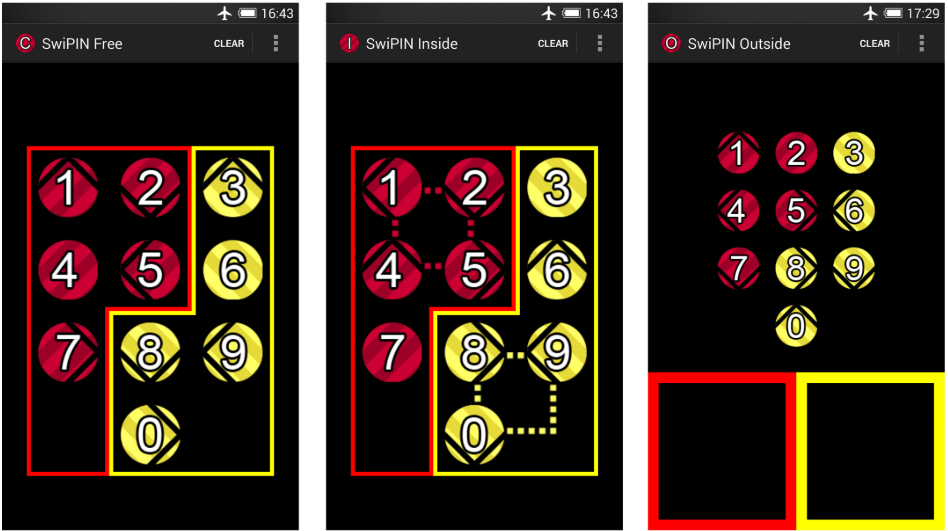
\includegraphics[width=13cm, height=7cm]{Chapters/graphics/swipin.PNG}
\caption{The three variations of \textbf{SwiPIN} by Zezschwitz et al. \cite{Swipin}. The version that was proven to be most usable is \textbf{SwiPIN} \textit{(outside}) on the far right \cite{Swipin}. }
\label{fig:swipin}
\end{figure}


\subsection{Approaches towards Novel Authentication Concepts} \label{2.2.3}

In addition to the previously discussed findings, researchers have also contributed towards proposing novel authentication methods. Although their intentions were primarily directed towards solving certain security issues, such as \textit{smudge} and \textit{shoulder surfing attacks} (see Chapter \ref{ch:first}), some of the authentication concepts have the potential of being more usable than the existing ones.\\

Zezschwitz et al. \cite{Swipin} created an authentication mechanism called \textbf{SwiPIN} (see figure \ref{fig:swipin}). It was intended to support the original \textit{pin} method in situations in which stronger authentication security is needed. Its main task was to prevent \textit{shoulder surfing attacks}. Zezschwitz et al \cite{Swipin} created three variations of the concept, of which \textbf{SwiPIN} \textit{(outside)} showed to have the best usability (see figure \ref{fig:swipin}). It is comprised of entering the pin through gestures rather than by tapping the buttons (numbers) on the screen. The interface presents a number pad, and on each of the buttons, there is a black arrow, which indicates the direction in which the gestures should be performed. Also, for each button, a specific color is assigned (\textit{yellow} or \textit{red}). To enter one's pin, one would simply perform the gestures of the respective numbers in one of two "boxes" displayed at the bottom of the screen. Gestures of red buttons are performed in the red box and gestures of yellow buttons, in the yellow box (see figure \ref{fig:swipin}). The black arrows, which are assigned to each number, change for each authentication run. This design increases the effort and memory needed to "successfully" perform a shoulder surfing attack because the attacker must try to memorize the gestures, their order, and the color of the boxes in which they are performed in order to obtain which numbers were entered. \\

\begin{figure}[t!]
\centering
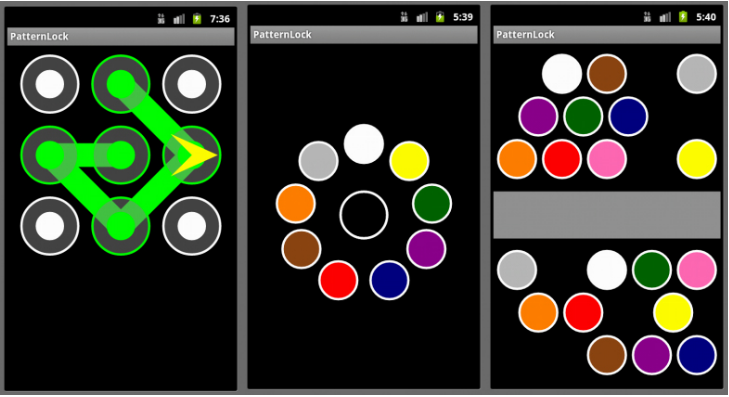
\includegraphics[width=13cm, height=7cm]{Chapters/graphics/graphic.PNG}
\caption{The three concepts made by Zezschwitz et al. \cite{Marbles}. (Left) Pattern 90, a special version of Pattern Rotation, (Middle) Marbles, (Right) Marble Gap, a variation of Marbles.}
\label{fig:marbles}
\end{figure}

Zezschwitz et al. \cite{Swipin} further conducted a study in which \textbf{SwiPIN} and the original \textit{pin} concept where compared to each other. They noticed that the utilization of \textbf{SwiPIN} lead to a slightly longer authentication process than \textit{pin}. A notable disadvantage of the concept \textbf{SwiPIN} was that users had to approach it differently than usual. Since entering a memorized pin into a number pad usually depends on muscle memory, users had to consciously recall their pin, while using \textbf{SwiPIN}. This lead to an increase of mental effort during utilization. Nonetheless, all participants of the study approved of the concept and imagined themselves using it in unsafe environments. \\

Another contribution towards designing novel security concepts was made by Zezschwitz et al. \cite{Marbles}. Their goal was to create a protection mechanism against \textit{smudge attacks}. They created three concepts: \textbf{Marbles}, \textbf{Marble Gap} and \textbf{Pattern Rotation} (see figure \ref{fig:marbles}). The idea for \textbf{Marbles} is to create an interface that presents colored dots (marbles) aligned in a circular order. The marbles represent the elements that define a specific password. In order to authenticate, the user would enter their password by dragging the marbles into the center circle in the right order. \textbf{Marble Gap} is based on the same idea, yet differs in its mapping (see figure \ref{fig:marbles}). The marbles are displayed at the top and bottom of the screen, separated by a centered rectangle (gap). To enter the password, the user would drag in the marbles into the gap, either from the top or bottom. It is important to note that the arrangement and display of the marbles were random for each authentication run in both concepts. \textbf{Pattern Rotation} is based on the traditional \textit{Android Unlock Pattern} mechanism. The interface presents a 3x3 grid of nodes, which changes its orientation every time a user wants to authenticate. A special version of \textbf{Pattern Rotation}, namely \textit{Pattern 90}, enables four different grid orientations: 90$^\circ$, 180$^\circ$, 270$^\circ$, and 360$^\circ$ (see figure \ref{fig:marbles}). \\

To examine which one of the three concepts users' preferred best in terms of efficiency and effectiveness, Zezschwitz et al. \cite{Marbles} conducted a study in which all three concepts were analyzed. They adopted a specific approach to measure the authentication times by dissecting the authentication process into \textit{orientation} and \textit{input} time. Harbach et al. \cite{AnatomySmartphone} made a similar approach when they analyzed the difference between \textit{pin} and \textit{pattern} (see Section \ref{2.2.2}). Zezschwitz et al. \cite{Marbles} defined the \textit{orientation} time as the period between the initiation of the authentication and the first input event, made by the user. \textit{Input} time was interpreted as the period between the first input event and the moment in which the input is either approved or rejected. Through this distinction, they realized that the factor of randomization in each of the concepts affected their overall authentication time in different ways. For instance, with \textbf{Marbles} and \textbf{Marble Gap}, randomization was shown to elongate the \textit{input time}, because the marbles were positioned differently in every authentication run, and so the user had to search for each marble before entering it. In contrast, the \textit{orientation time} of \textbf{Pattern Rotation} was increased through randomization because participants needed more time to familiarize themselves with the current position of the grid. Another discovery made, through the distinction of \textit{orientation} and \textit{input}, was participants' perception of speed. While \textbf{Pattern Rotation} was measured to be the second quickest of all three, participants rated it as the slowest. Nonetheless, \textbf{Pattern Rotation} had the longest measured \textit{orientation time}. This discovery allowed Zezschwitz et al. \cite{Marbles} to realize that users disliked mechanisms which had long \textit{orientation times}. Therefore, \textbf{Pattern Rotation} was considered not usable. Security analysis also showed that it was not sufficiently secure. In contrast, participants approved of \textbf{Marbles} and \textbf{Marbles Gap} and perceived them as very usable.

\section{Focus} \label{2.3}

In retrospect, the previously presented research contributions underline how crucial efficiency and effectiveness are for the user-acceptance of a particular authentication mechanism. Yet, the question remains, which of the two has the potential to achieve more successful and desired results, when enhanced. The following section will justify the author's choice of focus by elaborating on the potential effect of each factor, based on the related work (see Section \ref{2.2}). \\

Many instructive propositions were made towards improving effectiveness, from using social intervention methods, to specifically adapting the maintenance of smartphone security to users' country of origin (see Section \ref{2.2.1}). Although these propositions have a potential to cause improvement in usability, they are either only successful to a certain extent, or complicated to implement. For instance, when Albayram et al. \cite{Albayram:2017:BUL:3235924.3235929} used an educational video as a method of intervention, it was effective, yet the desired effect was only noticeable in 50\% of their treatment group. The other half of the group still persisted on not to use a screen lock on their smartphone. In addition, in order to implement the proposition made by Harbach et al. \cite{Harbach:2016}, one would need to study each country to specifically design smartphone authentication methods that satisfy the wants and needs of smartphone users around the world. This approach does not only require much time and many resources, yet it also is difficult to implement thus, realistically, all people differ in their wants and needs, despite their country of origin. So, it would be strenuous to create a smartphone authentication method that satisfies the majority of the people of a particular country. \\

On the contrary, people are similar in their instinctive behaviour. As mentioned in Section \ref{2.1.2}, humans are naturally prone to facilitate certain tasks or actions that appear complicated or unnatural to them, which is the case with current authentication methods. This implies that humans instinctively favor tasks and actions that are fast and easy to perform, and that are, therefore, efficient. Findings in Section \ref{2.2}, described that the primary reason why users persist to not use screen locks is because they perceive them as \textit{inconvenient}. Another study revealed that users prefer to use a screen lock if it delivers a faster performance than the existing ones. On that note, laying focus on increasing the efficiency of authentication mechanisms could be more productive towards the improvement of their usability. \\

However, creating authentication concepts that are fast and easy to use is not as intuitive as it seems. As Zezschwitz et al. \cite{PatternWild} compared two commonly used authentication mechanisms, \textit{pin} and \textit{pattern}, they noticed that their participants prefered using \textit{pattern} more that \textit{pin}. Reason being, that it handled errors better than \textit{pin} did, and that it needed less time for preparation. Nonetheless, time measurements showed that with \textit{pattern} participants needed more time to authenticate than with \textit{pin}. These results show that only focusing on time measurements to evaluate efficiency could lead to making false conclusions. Instead, human perception of time and speed should be used as the metric to do so. For that, research should be directed more specifically towards enhancing \textit{perceived efficiency}. Therefore, specific methods of approach are called for to observe the factors that affect the human perception of efficiency. \\

On that note, Zezschwitz et al. \cite{Marbles} compared newly developed authentication concepts by using a specific manner of approach. In noticing that preparation time played a role in the perceived efficiency of authentication mechanisms, they dissected the overall authentication time into \textit{orientation} and \textit{input} (see Section \ref{2.2.3}). Consequently they noticed that the concept which had the second shortest overall authentication time, was perceived least usable. The outcome was due to the concept's long \textit{orientation time}. Participants seemed to dislike this aspect of the authentication concept.\\
This observation arises the question on whether the length of \textit{orientation time} has an effect on the perceived efficiency of an authentication mechanism or not. A group of researchers contributed towards answering this question by proposing an extended method on improving perceived efficiency of authentication mechanisms by redefining the anatomy of a general authentication process. In Chapter 3, their work will be discussed in detail, thus it serves as the theoretical groundwork of this thesis. Although, in this section, efficiency was shown to outweigh effectiveness, based on the findings in Section \ref{2.2}, the solutions for enhancing effectiveness in authentication still remain important and useful and could be implemented as supportive solutions to further enhance usability in efficient authentication mechanisms.



